\section{Cubedate: Standard Security for Continuous Deployment of Low-power CubeSat Software}
\label{sec:low-power-orbital-communication-arch}

In this section we describe Cubedate, a structured approach to securing heterogeneous software updates for cubesat software in orbit.

\subsection{Security Requirements}
The minimal security guarantees that we aim for with Cubedate are authenticity and integrity of software updates delivered over the network, during the lifetime of the satellite mission (5-10 years).
As a matter of fact, a 10 years life span is a rather long time, during which cryptographic primitives used to secure software updates may have to evolve.
Thus Cubedate must allow for crypto agility: evolving the crypto primitives used to secure update to the satellite while in operation. This need can be dictated either by cryptography's evolving state-of-the-art (implementation/algorithm vulnerabilities are discovered) or by the need to transfer the trust anchor to a new entity (the authorized maintainer has changed).
Additional guarantees beyond authenticity/integrity should also be possible with Cubedate, such as confidentiality, software update replay attacks, or software update mismatch attacks.

\subsection{Trust Anchor}
Our model is based on a single trust anchor: the authorized maintainer for the cubesat hosted payload.
There is no mitigation if this trust anchor used is compromised. 
We thus rely on the maintainers' ability to keep their private keys secure. 
Extensions using a (hierarchical) public key infrastructure are possible but out of scope for this paper.

\subsection{Cubedate Software Life-Cycle Phases}
The basic process we use for securing authenticity and integrity of software updates is decomposed in six phases shown \autoref{fig:phases}. 

During a preliminary, pre-flight phase (\textit{Phase 0}) the authorized maintainer for the CubeSat-hosted payload
produces and flashes the payload with commissioning material:
a bootloader, the initial firmware, and authorized crypto material (a public key, and a cryptographically strong hash function).
Once the hosted payload is commissioned it can be sent to the CubeSat operator of installation in the CubeSat.

Once the CubeSat in orbit, the hosted payload maintainer can trigger iterations through cycles of Phases 1-5, whereby
the authorized maintainer can build a new software update (\textit{Phase 1}), hash the update
and sign the hash (\textit{Phase 2}) then push a network transfer (PUT) towards the hosted payload via the ground station and the OBC (\textit{Phase 3.1}). The next time it wakes up, the hosted payload can
then ping and fetch (GET) the update from the OBC (\textit{Phase 3.2}), proceed to verify the signature and the hash (\textit{Phase 4}),
and upon successful verification, install/boot the new software (\textit{Phase 5}), otherwise the update is dropped.

\begin{figure}[t]
    \centering
    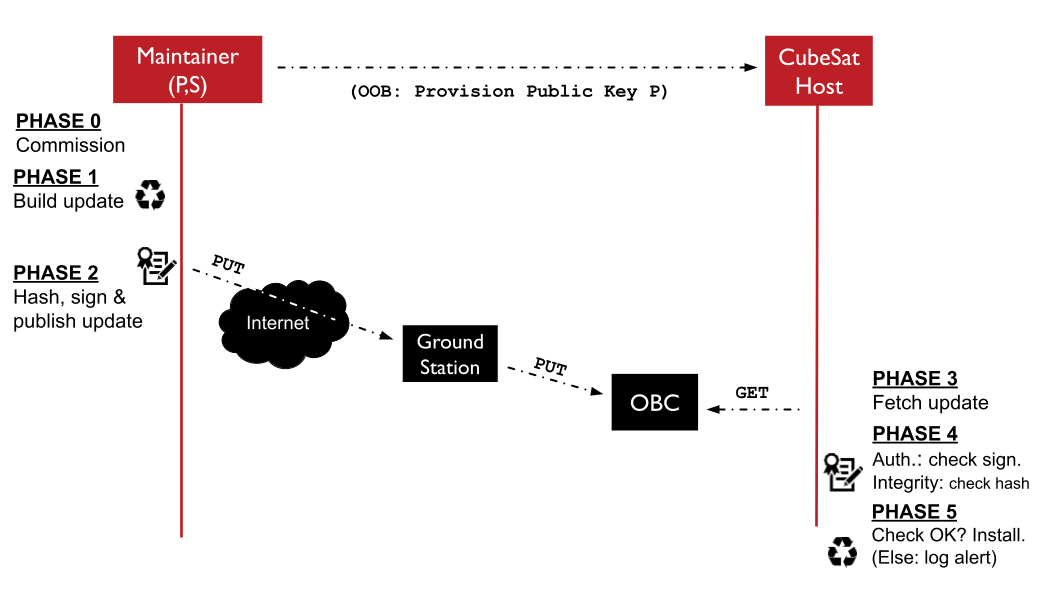
\includegraphics[width=0.5\textwidth]{Figures/CubeSat-Payload-update.png}
    \caption{CubeSat hosted payload secure software update process.}
    \label{fig:phases}
\end{figure}

\subsection{Supporting Network Transport Heterogeneity}
This aspect concerns \textit{Phase 3.1} and \textit{3.2} in \autoref{fig:phases}.  Security guarantees on software updates must remain valid "end-to-end".

Depending on the use-case "end-to-end" spans differently, as depicted for example in \autoref{fig:e2e}. In the most complex case we tackle in this paper, end-to-end means all the way from the hosted payload software maintainer to the payload hosted in orbit on the CubeSat.

Software updates may be transported over one or more network links of varying nature: 
\begin{itemize}
\item {\bf Developer to Groundstation}: via wired Internet, USB key upload...
\item {\bf Groundstation to CubeSat}: via long-range radio links such as UHF, LoRa...
\item {\bf Intra-CubeSat}: via bus communication such as CAN/CSP, SPI...
\item {\bf Path \& Delay Tolerance}: the end-to-end network path can either be a single link (simplest case) or a series of links which never exist simultaneously (most complex case) which may require temporary in-network caching.
\end{itemize}

\iffalse
Second, paths across the network may vary in complexity.
In the simplest case the end-to-end network path covers consists in a single segment: from a ground station either to the OBC, or to the hosted payload directly via its own radio interface, if it has one (as described in \autoref{sec:thingsat-comm-characteristics}).
In more complex cases involving hosted payloads, not only
must the end-to-end path traverse multiple heterogeneous network segments,
but also: this path may never exist end-to-end at any point in time.
This Delay-tolerant network characteristic is due to power-off periods imposed on CubeSat hosted payloads, 
combined with fact that CubeSat are out-of-range for ground stations radios a large part of the time.
Hence, while in transit across the network, software update data may have to be temporarily cached at some intermediate node along the path.
\fi

To cope with this wide variety of network paths and links (including ultra-constrained low-power elements), different approaches can be envisioned at the network layer, the transport layer and the application layer. Approaches span from proprietary solutions to standards such as the low-power IPv6 protocol stack (6LoWPAN, UDP, CoAP \cite{morabito2020ietf}) or experimental stacks such as information-centric networking which benefits from in-network caching even with small caches on microcontrollers \cite{hahm2017low}. 

Nevertheless, in order to retain generality, Cubedate does not specify any particular approach at the network, transport and application layers to enable the delivery of software updates across the network.
Cubedate only aims to guarantee end-to-end security properties for the software update binaries that are delivered, somehow, over the network.

\subsection{Supporting Updated Software Heterogeneity}
This aspect concerns both \textit{Phase 1} and \textit{Phase 5} in \autoref{fig:phases}. 
As seen in \autoref{sec:thingsat-update-req}, software updates may be of various nature and size.
Cubedate aims to support the same mechanism, workflow and guarantee to update the cubesat (1) firmware updates, (2) mission scenario files and (3) runtime configuration files.

For this reason, we choose not to rely on specialized approaches such as DFU (Device Firmware Update \cite{beningo2018dfu}) which assumes that the software is firmware and that the device is connected directly via some local bus connection (e.g. USB).

Instead, we aim to combine the use of generic and standard metadata characterizing software updates and state-of-the-art cryptographic primitives applicable on most low-power microcontrollers and a large variety of low-power networks, as described below.

\subsection{Low-power End-to-End Security using SUIT}

Cubedate leverages the SUIT manifest~\cite{suit-manifest} which specifies a metadata format to describe software updates. This format uses Concise Binary Object Representation (CBOR) for data serialization, and a security wrapper which protects the metadata end-to-end, leveraging the CBOR Object Signing and Encryption (COSE) specification -- all of which are IETF open standards for low-power communication security~\cite{tschofenig2019cyberphysical}.

The Cubedate software update binary itself can be either encapsulated in the SUIT manifest, or transferred separately based on the URI provided in the manifest.
For instance, the metadata includes a sequence number (preventing unwanted rollbacks), the expected device type (preventing software mismatch), the SHA256 digest of the software update binary, and the ed25519 digital signature of the manifest (the metadata).
\todoEB{Add more specific parameters we use with/for SUIT for Cubedate?}
As such, using Cubedate, software updates for payload hosted on CubeSats mitigate attacks including:

\begin{itemize}
\item {\bf Tampered Software Update Attacks –} An attacker may try to update the IoT device with a modified and intentionally flawed software image. To counter this threat, Cubedate uses digital signatures on a hash of the image binary and the metadata to ensure integrity of both the firmware and its metadata.

\item {\bf Unauthorized Software Update Attacks –} An unauthorized party may attempt to update the IoT device with modified image. Using digital signatures and public key cryptography, Cubedate ensures that only the authorized maintainer (holding the authorized private key) will be able to update the device.
\end{itemize}

\subsection{Supporting Crypto Agility}
The first level of crypto agility enabled by Cubedate uses flexibility provided by the SUIT standard specification: while keeping the same metadata and workflow, diverse crypto primitives backends can be used. For instance, to upgrade from pre- to post-quantum security, digital signature performed with ed25519 (elliptic curve crypto), can be swapped for hash-based signatures (LMS~\cite{banegas2022quantum-suit}).

The second level of crypto agility enabled by Cubedate leverages a dedicated embedded runtime architecture as shown on the Flash memory layout depicted in \autoref{fig:cubedate-runtime}. On the one hand, we place the software update manager (implementing SUIT-related operations) in the firmware image itself. On the other hand, we perform cryptographic operations in software only.

Thus, changing the trust anchor stored is as simple as swapping a public key in the next firmware's update manager.
Authorization to update the firmware can thus be easily  delegated to another maintainer, 
who can take over the production and the roll out of authorized updates.
Furthermore, the update manager in the next firmware image could
implement and use upgraded cryptographic primitives. 

\begin{figure}[t]
\begin{center}
    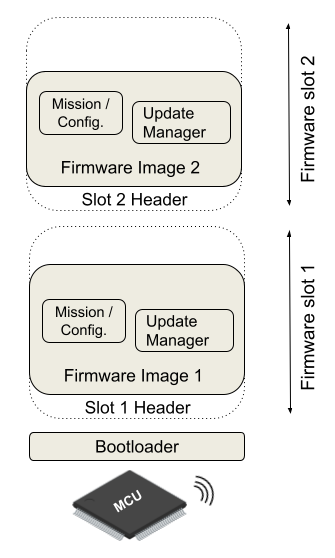
\includegraphics[width=0.25\textwidth]{Figures/Cubedate-slots.png}
    \caption{Flash memory layout of the Cubedate runtime.}
    \label{fig:cubedate-runtime}
\end{center}
\end{figure}

\subsection{Guarantees beyond Authenticity/Integrity}

Cubedate may also guarantee confidentiality by encrypting (optional) software updates transmitted over the network.
It is performed using the encrypt/decrypt mechanism provided by the SUIT specifications~\cite{suit-firmware-encryption}, using a symmetric cryptographic key commissioned in the update manager by the authorized maintainer. 
Confidentiality can mitigate additional cyberattacks leveraging analysis of cubesat firmware/software binaries.

Going beyond authenticity, integrity and confidentiality guarantees for software updates delivered over the network, using Cubedate also mitigates other attacks including:
\begin{itemize}
\item {\bf Software Update Replay Attacks –} An attacker may try to replay a valid, but old (known-to-be-flawed) software. This threat is mitigated by using a sequence number. Cubedate uses a sequence number, which is increased with every new software update.

\item {\bf Software Update Mismatch Attacks –} An attacker may try replaying a software update that is authentic, but for an incompatible device. Cubedate includes device-specific conditions, which can be verified before installing a software binary, thereby preventing the device from attempting to use an incompatible software image.
\end{itemize}
